\documentclass[10pt, conference, compsocconf]{IEEEtran}
\hyphenation{op-tical net-works semi-conduc-tor}
\usepackage{amsmath}
\usepackage{CJK}
\usepackage{algorithm}
\usepackage{algorithmic}
\usepackage{color}
\usepackage{stfloats}
\usepackage{supertabular,booktabs}
\usepackage{graphicx}
\usepackage{bm}
\usepackage{cite}
\usepackage{biblatex}
\addbibresource{references.bib}
\usepackage[colorlinks,linkcolor=red,anchorcolor=blue,citecolor=green,CJKbookmarks=True]{hyperref}
\begin{document}
\begin{CJK}{UTF8}{gbsn}
\title{基于离散选择模型的结直肠癌筛查偏好研究}
\author
{\IEEEauthorblockN{苏锦华 \IEEEauthorrefmark{1}}
\IEEEauthorblockA
{
\IEEEauthorrefmark{1}中国人民大学统计学院\\
}
$ $\\
$\{2017201620\}@ruc.edu.cn$
}

\maketitle

\begin{IEEEkeywords}
癌症筛查偏好;DCE;多元logit模型
\end{IEEEkeywords}


\IEEEpeerreviewmaketitle
\section{相关研究}
为更好地开展癌症筛查工作,政策制定者需了解目标人群的筛查偏好,找到并权衡影响其参加癌症筛查的属性(如筛查效果),这是设计与实施科学合理筛查方案的关键。

陈述性偏好(stated preference)方法利用离散选择实验 (discrete choice experiments,DCEs)研究目标人群癌症筛查偏好,系统分析影响其参加癌症筛查的重要因素\parencite{刘童童离散选择实验用于癌症筛查偏好的国际研究进展}。



DCE对被调查对象的分析基于随机效用理论 (random utility theory)\parencite{宋奎勐利用离散选择实验研究卫生服务人员工作偏好的国际研究进展}。在构建回归模型时,将筛查方案是否被受访者选中作为因变量,癌症筛查属性作为自变量。由于因变量是哑变量的属性,logit或probit模型常用于估计目标人群对各个癌症筛查属性的效用值,从而得到筛查方案总的效用值。

有关 DCE 的研究大多采用随机效果 probit 模型(random effects probit)、条件logit模型 (conditional log⁃it)、多项式 Logit 模型 (multinomial logit) 等经典模型;近年来,嵌套 logit 模型 (nested logit)、混合 logit模型 (mixed logit,考虑了受访者的选择异质性\parencite{milte2014cognitive}(preference heterogeneity))、广义多项式 logit 模型 (gener⁃alised multinomial logit,同时考虑了受访者的选择异质性和规模异质性\parencite{kjaer2008preference} (scale heterogeneity))也逐渐成为研究人员开展DCE研究所采用的模型。
% \begin{itemize}
% \item 自动地从几个具有影响力的财经网站下载新闻;
% \item 对从网站中爬取的新闻进行分词等预处理;
% \item 构建一套无监督标注方法来近似正负情感的标注;
% \item 使用BERTtokenizer对预处理文本数据进行表征处理,使用伪标注数据进行训练;
% \item 使用训练好的BERT模型对近期未标注的数据进行预测,计算每天的新闻计算当天的舆情得分;
% \item 选择合适的标准对舆情因子与市场趋势的相关性进行分析,评价舆情因子是否对金融投资有帮助。
% \end{itemize}
% 文章剩下的部分安排如下:第二部分描述研究的背景和相关研究,包括结巴分词,BERT和Finetuning。第三部分包括实验结果和讨论。最后第四部分则是我们的结论。


% \begin{figure}[ht]
% \centering
% \includegraphics[scale=0.12]{bert.jpg}
% \caption{BERT模型结构与GPT,ELMO模型结构的对比}
% \end{figure}

\section{数据}
\vspace{0.5cm}
\subsection{\underline{数据处理}}
回收网络问卷525份,问卷设置了10道个人特质问题,3大类方案,其中选择方案是3种属性的组合。由于对不同个体,不同医院来说,三类选择方案中风险降低程度、复查频次是不存在唯一的客观值,通过改变风险、频次得到18种假设情景供受访者选择。

将每一种假设情景作为一条数据,每份问卷实际上可分成18条供模型训练的数据,总计9449条训练数据,数据变量取值与含义如下。
\begin{table}[h]
\caption{数据变量解释}\label{Table 2}
\centering
\begin{tabular}{p{1cm}p{7cm}}
% \begin{tabular}{c|c}
\hline
sex & 性别:0表示男,1代表女 \\
age & 年龄:0~3表示50周岁到70周岁(5岁一挡),4表示70周岁以上\\
income & 年收入:0表示五万一下,1表示5-10万,2表示10万以上\\
region & 居住地区:0表示乡镇,1表示市区\\
edu & 学历:0表示初中及以下,1表示高中及中专,2表示本科及大专,3表示研究生以上\\
work & 就业状态:1表示工作,0表示不工作\\
retire & 退休状态:1表示退休,0表示尚未退休\\
chronic & 是否有慢性病史:1表示是,0表示否\\
check & 是否做过结直肠检查:1表示是,0表示否\\
hospital & 是否有过住院经历:1表示是,0表示否\\
attention & 健康关注程度:0~4健康关注程度逐步提高\\
risk\_dec & 筛查方案风险降低百分比(\%)\\
frequency & 筛查方案每隔x年需复查\\
pain & 筛查方案检查机器深入肠道的长短(cm)\\
choice & 筛查方案选择:0表示粪便潜血试验,1表示乙状结肠镜,2表示全结肠镜\\
\hline
\end{tabular}
\end{table}

\subsection{\underline{数据描述}}

对9449条数据的各属性分别统计频次直方图。总体上三套方案选择人数相近,乙状结肠镜的筛查方案稍微低于另外两套方案。个人特征属性的数据分布情况各异:年龄分布上50-60岁人数居多,对健康的重视程度普遍较高,直结肠检查比例大致80\%,慢性病比例70\%,受教育程度平均为高中教育,选择复查间隔较短的人数较多,有住院经历的占60\%,80\%的人群年收入在5万以下,65\%的人群居住在城市,55\%的受访者尚未退休,65\%的受访者为女性,大部分受访者更青睐风险降低程度较大的方案。
\begin{figure}[ht]
\centering
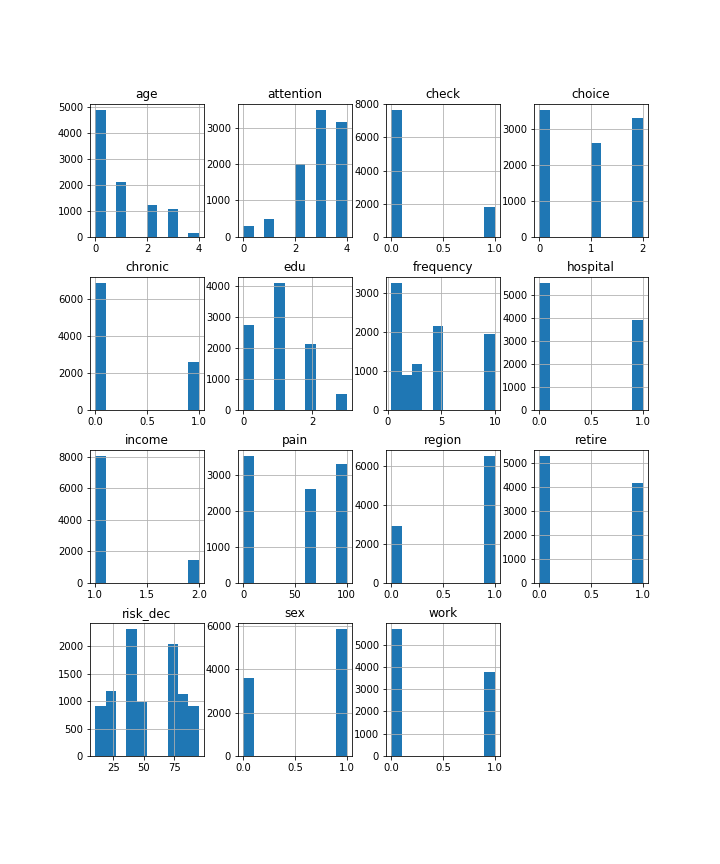
\includegraphics[scale=0.35]{hist.png}
\caption{数据直方图}
\end{figure}

\section{模型}
\vspace{0.5cm}
本文选择多元逻辑回归来探究不同因素对筛查方案选择偏好的影响。因素分为个人特征因素与选择情景因素,本文构建了普通多元logit模型和带交互项的多元logit模型。普通多元logit模型假设各因素间相互独立互不影响,而带交互项的多元logit模型考虑个人特征对偏好的复合影响。

为了使模型具有较好的解释性,本文通过前进法依次选取对模型影响最显著的变量纳入模型,去除共线性较高使得模型训练难以收敛的变量。
\subsection{\underline{多元logit模型}}
\subsubsection{\underline{模型公式}}
U是基于随机效用假设的效用,n代表第n个样本,j代表第j个选择方案,s代表选择情景,在本文中代表风险和频次不同的18个假设情景。V为多元logit模型估计的效用值,选择第j个方案概率是所有方案效用的softmax值。
\begin{equation}
U_{njs} = \beta_j x_{njs} + \epsilon_{njs}
\end{equation}

\begin{equation}
V_{njs} = \beta_j x_{njs}
\end{equation}

\begin{equation}
Pr_{njs}(\beta) = \frac{e^{\beta_j x_{njs}} } {\sum_{i=1}^J e^{\beta_i x_{nis}}}
\end{equation}
\subsubsection{\underline{前进法选择变量}}
本文选择了前进法选择前10个变量拟合多元logit模型。在假设情景数据中,频次的影响最显著,风险降低的影响不显著,pain由于在不同情景中未发生变化,存在与choice较高的共线性未被选入。收入、性别、教育、工作情况对偏好的影响较显著,而年龄、就医经历、病史、对健康的重视程度则对偏好的影响不显著。
\begin{table}[h]
\caption{模型一前进法选择结果}\label{Table 2}
\centering
\begin{tabular}{p{7cm}}
% \begin{tabular}{c|c}
\hline
$frequency >> intercept >> income >> sex >> edu >> work >> retire >> check >> hospital >> age >> chronic >> region >> risk\_dec >> attention$
\hline
\end{tabular}
\end{table}

\begin{figure}[ht]
\centering
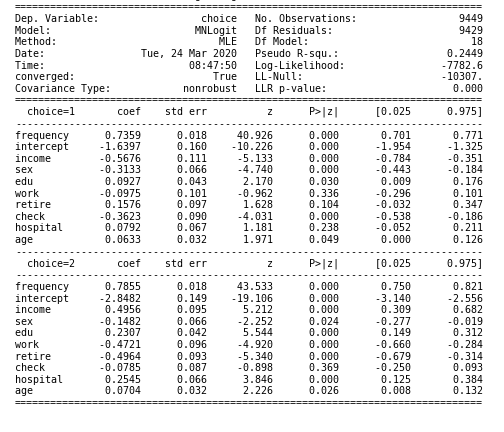
\includegraphics[scale=0.5]{res1_10.png}
\caption{多元logit模型}
\end{figure}


\subsection{\underline{带交互项的多元logit模型}}
\subsubsection{\underline{模型公式}}
在普通多元logit模型中,beta是需要拟合客观数值。现实情况中不同的个人特征对方案偏好有影响,本文模型二假设beta是个人特征属性的线性加性函数,将公式(5)带入公式(4)可以得到个人属性与情景属性的交互项。
\begin{equation}
U_{njs} = \beta^{'}_{j}(character) situation_{njs} + \epsilon_{njs}^{'}
\end{equation}

\begin{equation}
\beta_{j}^{'}(character) = \beta_{j0}^{'} + \beta_{j1}^{'}sex + \beta_{j2}^{'}age + ...
\end{equation}

\subsubsection{\underline{前进法选择变量}}
本文选择了前进法选择前15个变量拟合带交互项的多元logit模型。频次依旧是最显著的影响因素,其他被选入的重要变量均为交互项,剩余的较重要的非交互项只有受教育程度,说明不同个人特征的确对筛查偏好的选择有重要影响。含有收入、对健康的重视程度、是否工作与退休、受教育程度、年龄的交互项较显著,说明以上个人特质属性对筛查偏好有重要影响。
\begin{table}[h]
\caption{模型二前进法选择结果}\label{Table 2}
\centering
\begin{tabular}{p{7cm}}
% \begin{tabular}{c|c}
\hline
$frequency >> intercept >> income*risk_dec >> income*frequency >> attention*risk\_dec >> attention*frequency >> retire*risk_dec >> retire*frequency >> work*risk\_dec >> work*frequency >> edu >> edu*frequency >> age*risk\_dec >> age*frequency >> sex*pain >> chronic*risk\_dec >> region >> chronic*frequency >> region*frequency >> hospital*risk\_dec >> chronic*pain >> region*risk\_dec >> check*frequency >> check*risk\_dec >> check*pain$
\hline
\end{tabular}
\end{table}

\begin{figure}[ht]
\centering
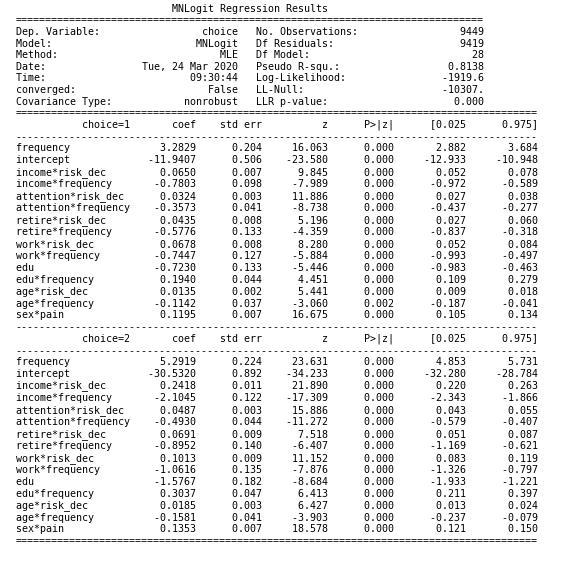
\includegraphics[scale=0.4]{res2_15.png}
\caption{带交互项的多元logit模型}
\end{figure}
% \begin{equation}
% distance = \frac{w_{1}\cdot w_{2}}{\|w_{1}\|\|w_{2}\|} = w_{1}^{'}\cdot w_{2}^{'}
% \end{equation}








\vspace{0.5cm}

\section{\underline{结论}}
模型有三个选项,以choice=0对基准,分别对剩余两个变量进行logit回归,其系数正负与大小均以choice=0的系数为0作为基准。
\section{\underline{模型一拟合结果解读}}
频率拟合系数均为正向高度显著,且choice=2>choice=1系数,说明复查间隔越大,第三个方案的边际对数效用提升最大,其次是第二个。可以理解当复查间隔越长,二三方案更可能被选择。

choice=1收入影响是负向显著,choice=2收入影响是正向显著,说明当收入越高,越可能选择方案三,其次是方案一,选择方案二的概率减少。

性别的影响系数均为负向显著,且choice=1负值程度更大,说明女性相比男性更倾向与选择方案一,对方案二的拒绝程度比方案三更大。

教育的影响系数均为正向显著,且choice=2系数数值更大,说明受教育程度高的人更倾向于选择方案三,其次是方案二。

是否工作与是否退休的拟合系数的均仅有choice=2显著,都为负无论工作还是退休都更愿意选择方案一而非方案三。

是否经历过直结肠检查的系数仅有choice=1显著为负,说明经历过直结肠检查的人对方案三既不偏好也不厌恶,而在方案一与方案二中更愿意选择方案一。

是否有住院史的系数仅有choice=2显著为正,说明有住院史的人在方案一与方案三中更愿意选择方案三,对方案一和方案二则没有明显差别。

年龄系数均为正向显著,choice=2数值更大,说明年龄越大,越倾向于选择方案三,其次是方案二。

\section{\underline{模型二拟合结果解读}}
频率拟合系数规律仍然同模型一解读,差别是方案三和方案二的边际偏好差值更大了。

收入与风险降低的交互系数均为正向显著,且choice=2数值更大,说明收入不同的人群对风险降低的效用感是不同,收入更高的人群对风险降低的偏好更大。

收入与频率拟合的系数可能存在与频率系数的共线性,缺乏解读意义,正是因为这种共线性,模型二的系数数值明显大于模型一。

对健康重视程度更高的人群、退休人群、年龄较高的人群均表现出和高收入人群相同的偏好变化,即更倾向于风险降低程度更高的方案,更偏好方案三而非方案二。而对频率的重视程度也呈现负值,也是由于与频率系数的共线性。

值得注意的是模型一中未被选入pain属性在模型二中与性别属性的交互呈现显著,说明女性比男性对深入直结肠的长度更加在意。

\printbibliography
\end{CJK}
\end{document}


